\subsubsection{Des médias négligents.}
La négligence et l'unicité des médias fait que les Fake News peuvent se propager facilement.
Comme nous l'avons dit précédemment, les médias traditionnels traversent une crise.
La production de contenus doit être faites le plus rapidement possible.
Dans le but de répondre à la course à l'information de plus en plus grande et déloyale, la qualité des articles est revue à la baisse.
Certains journalistes ne font pas le travail de vérifier leurs sources pour accélérer le procédé de publication.



\subsubsection{Des organisations malveillantes internationales.}
L'appât du gain facile que sont les Fake News a suscité des vocations.
En Macédoine, une partie de la jeunesse de Vélès s'est ainsi spécialisée dans la création de Fake News, attirée par de juteux revenus publicitaires. La ville s'est transformée en fabrique à Fake News pendant l'élection américaine\footnote{D'après le \href{http://www.lefigaro.fr/actualite-france/2017/03/06/01016-20170306ARTFIG00187-fake-news-un-meme-terme-pour-plusieurs-realites.php}{Figaro} 20/12/2017 }.
Mais aussi des sites comme \href{https://www.infowars.com/}{InfoWars} voient naître des Fake News.

\begin{center}
 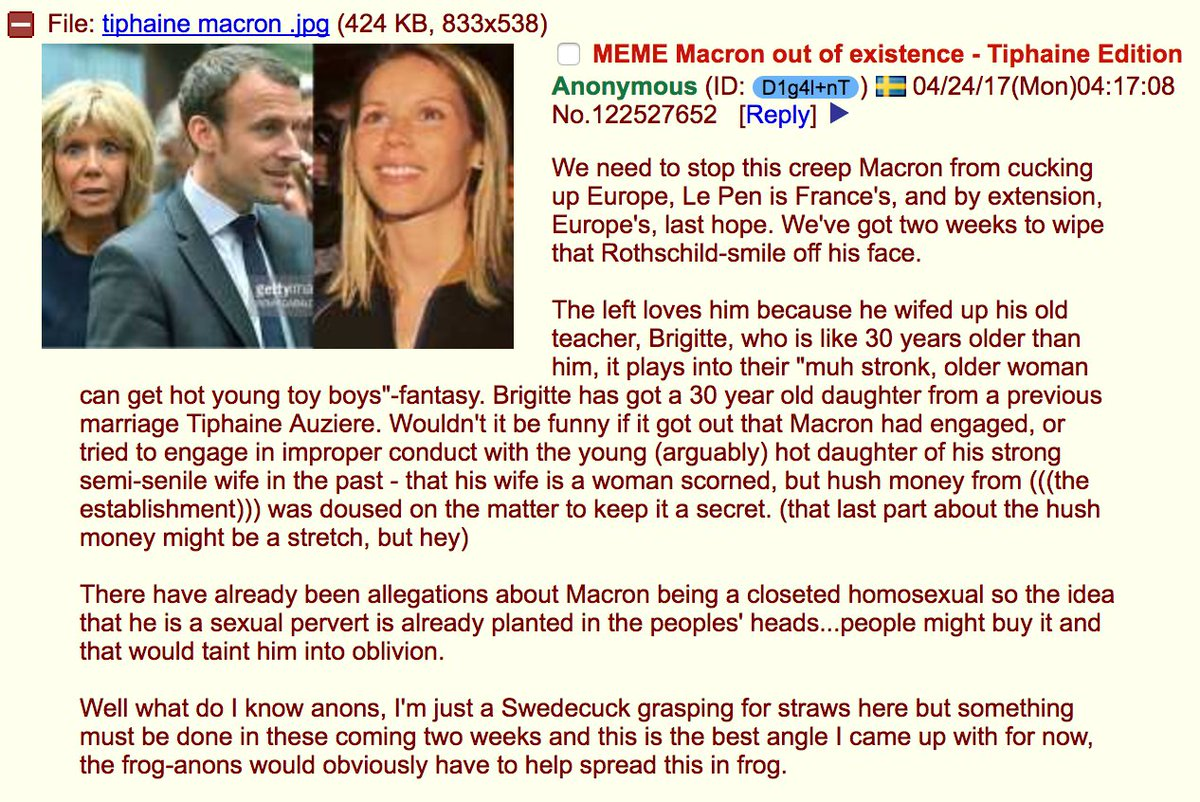
\includegraphics[scale=0.20]{../../img/rumeur_4chan/macron.jpg}
 \captionof{figure}{Capture d'écran d'un fil de discussion sur 4chan pour lancer une rumeur de pédophilie sur Macron.}
 \label{macron}
\end{center}

Des organisations qui travaillent dans l'ombre des plus grands forums sont à la base de la conception des Fake News.
En effet, l'étude de \href{https://arxiv.org/abs/1705.06947}{Savvas Zannettou et al, 2017} montre comment les forums leaders mondiaux que sont 4chan et reddit sont en partie responsable dans la création de rumeurs.
